
\chapter{Risoluzione delle DDE}
\vspace{1cm}
Si considerino le DDE 
$$
\begin{cases}
 y'(t) = f(t,y(t),y(t- \tau (t,y(t)))	\hspace{1cm}	t_0 \le t \le t_f \\
 y(t)=\phi(t)				\hspace{5cm}	t \le t_0
\end{cases}
$$
con
\begin{itemize}
 \item $f$ continua e lipschitziana sugli ultimi due argomenti
 \item $\tau$ (la funzione ritardo) non negativa, continua e lipschitziana sull'ultimo argomento
 \item $\phi$ (la storia) continua e lipschitziana
 \item l'intervallo in cui è definito il problema compatto
\end{itemize}

Sotto queste ipotesi la soluzione esiste ed è unica (è possibile 
indebolire queste ipotesi ma in questo contesto è inopportuno).
Si mostreranno due metodi per risolvere questi problemi, entrambi riconducono il problema 
di risolvere una DDE a quello di risolvere problemi ai valori iniziali che d'ora in avanti 
saranno saranno denotati con l'acronimo IVP (initial value problem).



\section{Metodo di Bellman}
Si consideri la DDE con ritardo costante
$$
\begin{cases}
 y'(t) = f(t,y(t),y(t- \tau))		\hspace{2cm}	t_0 \le t \le t_f \\
 y(t)=\phi(t)				\hspace{5cm}	t \le t_0
\end{cases}
$$
È possibile determinare la soluzione di tale problema nell'intervallo 
$[t_0,t_0+\tau]$ impostando un IVP
$$
\begin{cases}
 y'(t) = f(t,y(t),\phi(t- \tau))			\hspace{2cm}	t_0 \le t \le \tau \\
 y(t_0)=\phi(t_0)				
\end{cases}
$$
Per determinare la soluzione nell'intervallo successivo $[t_0+\tau , t_0 + 2 \tau]$ si definisce 
$y_1(t)=y(t-\tau)$ mentre $y_2(t)=y(t)$ quindi si imposta un IVP con dimensione doppia
$$
\begin{cases}
 y_1'(t)=f(t-\tau, y_1(t),\phi(t-2 \tau))				\\
 y_2'(t)=f(t,y_2(t),y_1(t))						\\
 y_1 (t_0 + \tau) = \phi(t_0)						\\
 y_2 (t_0 + \tau) = y(t_0+\tau)
\end{cases}
$$
In generale per trovare la soluzione nell'intervallo $[t_0+(k-1)\tau,t_0+k \tau]$ si dovrà risolvere 
un IVP con dimensione $k$ volte quella della DDE iniziale
$$
\begin{cases}
 y_i'(t)=f(t-(k-i) \tau, y_i(t), y_{i-1}(t)) \\
 y_i(t_0+(k-1)\tau) = y(t_0 + (i-1) \tau)
\end{cases} \hspace{1cm}
1 \le i	\le k
$$
Il processo termina quando si giunge a $k \tau \geq t_f$.

\vspace{0.4cm}

Con questo metodo è sufficiente esser in grado di risolvere gli IVP.\\
Il metodo è stato mostrato nel caso dei ritardi costanti ma è possibile generalizzarlo.

\vspace{0.3cm}

E' evidente che il costo computazionale è proibitivo dato che è necessario risolvere 
IVP a dimensione sempre più grande, quindi questo metodo può esser conveniente nel caso in cui 
il ritardo sia grande e l'itervallo in cui si vuole approssimare la soluzione sia piccolo.



\section{Metodo dei passi}
\subsection{Ritardo costante}
Si consideri la DDE
$$
\begin{cases}
 y'(t) = f(t,y(t),y(t- \tau))		\hspace{2cm}	t_0 \le t \le t_f \\
 y(t)=\phi(t)				\hspace{5cm}	t \le t_0
\end{cases}
$$
Si voglia determinare la soluzione nell'intervallo $[t_0,t_0+\tau]$, 
dato che in questo intervallo  
si ha che $t-\tau \in [t_0 - \tau, t_0]$ è possibile trasformare il problema in
$$
\begin{cases}
 y_1'(t) = f(t,y_1(t),\phi(t- \tau))		\hspace{3cm}	t \in [t_0 ,t_0+ \tau] \\
 y_1(t_0)=\phi(t_0)
\end{cases}
$$
e quest'ultimo è un IVP, risolto questo è possibile determinare la soluzione in 
$[t_0 + \tau, t_0 + 2 \tau]$, infatti si avrà un nuovo IVP
$$
\begin{cases}
 y_2'(t)=f(t,y_2(t),y_1(t-\tau)) 	 \hspace{2cm}			t \in [t_0+\tau,t_0 + 2\tau]	\\
 y_2(t_0+\tau)= y_1(t_0+\tau)
\end{cases}
$$ 
chiaramente la soluzione $y(t)$ in $[t_0,t_0+2\tau]$ sarà l'incollamento di $y_1(t)$ e $y_2(t)$, in generale 
per avere $y(t)$ nell'intervallo $[t_0,t_0 + N \tau]$ si dovranno risolvere $N$ IVP
$$
1 \le i \le N \hspace{1cm}
\begin{cases}
 y_i'(t)=f(t,y_i(t),y_{i-1}(t-\tau)) 	\hspace{1cm}  \hspace{1cm}		t \in [t_0+(i-1)\tau,t_0 + i\tau]	\\
 y_i(t_0+(i-1)\tau)= y_{i-1}(t_0+(i-1)\tau)
\end{cases}
$$
dove si pone $y_0(t):=\phi(t)$, e chiaramente $y(t)$ sarà l'incollamento di $y_1(t), \dots, y_N(t)$, ovvero

$$y(t)=y_i(t)	\hspace{1cm}	\mbox{se}	\hspace{1cm}	(i-1) \tau \le t \le i \tau$$

\begin{exm}
Si consideri la seguente DDE
$$
\begin{cases}
 y'(t)=-y(t-1)		 	\hspace{1cm} 		t \in [0,T]	\\
 y(t)=1				\hspace{2.5cm}		t \le 0
\end{cases}
$$
Usando il metodo dei passi, si determina la soluzione in $[0,1]$ , 
in questo caso si ha l'IVP
$$
\begin{cases}
 y_1'(t)=-1		 	\hspace{1cm}		t \in [0,1]	\\
 y_1(0)=1 
\end{cases}
$$
che ha come soluzione $y_1(t)=1-t$. Nell'intervallo $[1,2]$ si ha
$$
\begin{cases}
 y_2'(t)=t-2		 	\hspace{1cm}		t \in [1,2]	\\
 y_2(1)=0 
\end{cases}
$$
Cha ha come soluzione $y_2(t)=\frac{t^2}{2}-2t  + \frac{3}{2}$.
% sostituire immagine6
\begin{figure}[h]
\centering
\caption{Grafico della soluzione con T=10}
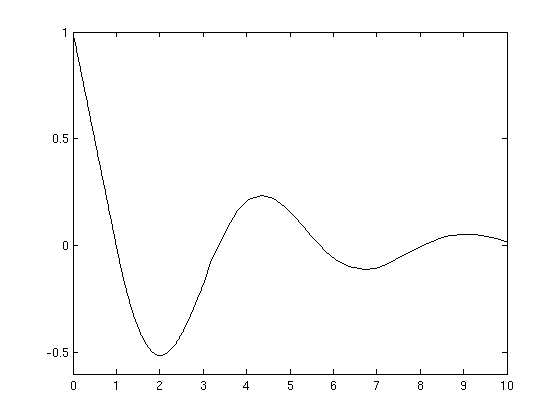
\includegraphics[width=11cm]{immagini/immagine6.png}
\end{figure}
Andando avanti si trova la soluzione su tutto $[0,T]$.
\end{exm}
\vspace{1cm}
\begin{oss}
 Si prenda in considerazione l'esempio appena fatto per fare un confronto tra IVP e DDE.
 $$
\begin{cases}
 y'(t)=-y(t-\tau)		 	\hspace{1cm}		t \in [0,T]	\\
 y(t)=1					\hspace{2.5cm}		t \le 0
\end{cases}
$$
Se il ritardo $\tau$ è nullo allora il problema è un IVP e di cui si conosce già che la soluzione $x(t)=e^{-t}$.
Una proprietà importante di questa funzione è che asintoticamente va a zero. \\
Introducendo un ritardo non trascurabile è lecito chiedersi se questa proprietà si conserva
% sostituire immagine8
\begin{figure}[h]
\centering
\caption{Grafici al variare del ritardo}
\subfigure[$\tau=0,T=5$]{
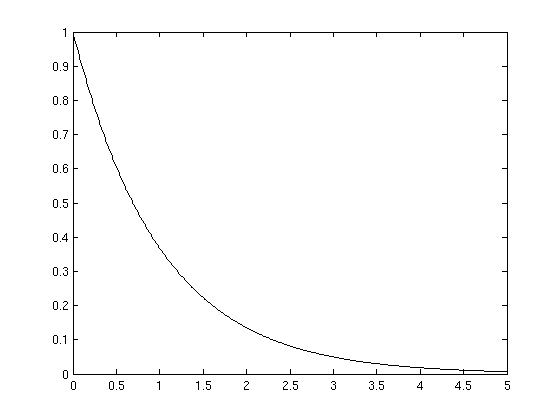
\includegraphics[width=4cm]{immagini/immagine7.png}}
\hspace{1mm}
\subfigure[$\tau=1,T=20$]{
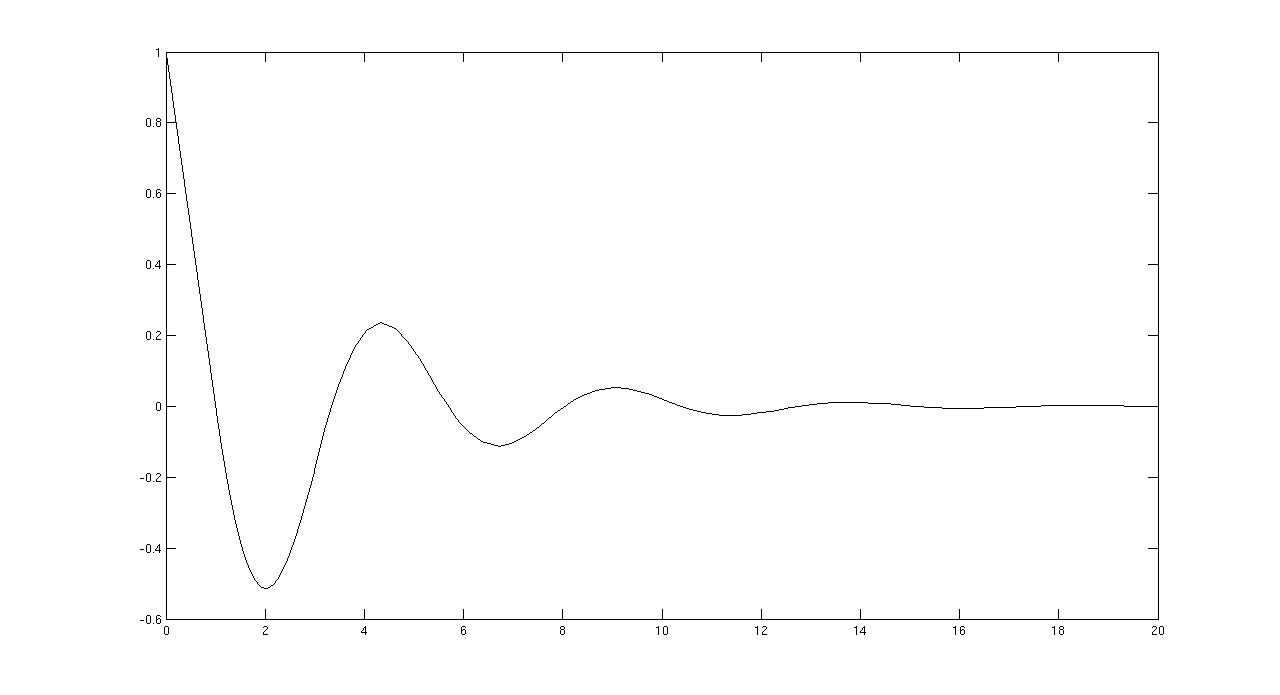
\includegraphics[width=5.6cm]{immagini/immagine8.png}}
\hspace{1mm}
\subfigure[$\tau=2,T=50$]{
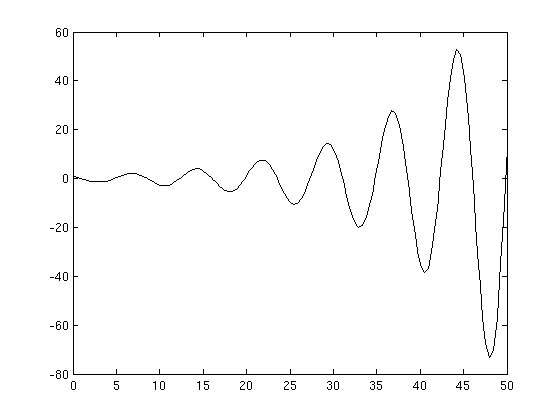
\includegraphics[width=4cm]{immagini/immagine9.png}}
\end{figure}\\
Come è possibile vedere dai grafici (e non è difficile dimostrarlo formalmente) se il ritardo 
non è troppo grande la soluzione continua a tendere a zero (a limite oscillando), ma se 
il ritardo diventa troppo grande (ad esempio $\tau=2$) la soluzione inizia ad oscillare divergendo.
Ciò intuitivamente fa pensare all'esistenza di diagrammi di biforcazione.
\end{oss}

\subsection{Ritardo variabile}
Si consideri una DDE con ritardo non costante
$$
\begin{cases}
 y'(t) = f(t,y(t),y(t- \tau (t,y(t)))	\hspace{1cm}	t_0 \le t \le t_f \\
 y(t)=\phi(t)				\hspace{5cm}	t \le t_0
\end{cases}
$$
data la suddivisione
$$
\Delta= \left \{ t_0, t_1, \dots , t_n , \dots , t_N = t_f \right \}
$$
risolvere la DDE equivale a risolvere $N$ problemi ai valori iniziali
$$
\begin{cases}
 w_{n+1}'(t)= f \left(t, w_{n+1}(t), x(t-\tau(t,w_{n+1}(t))) \right)	\hspace{0.5cm}	t_n \le t \le t_{n+1}	\\
 w_{n+1}(t_n)=y_n
\end{cases}
\hspace{1cm}
n=0, \dots, N-1
$$
dove si pone
$$
y_n:=y(t_n)	\hspace{2cm}
x(s):=
\begin{cases}
 \phi(s)	\hspace{2.2cm}	s \le t_0			\\
 w_{i}(s)	\hspace{1cm}	t_{i-1} \le s \le t_i 	
\end{cases}
$$

Supponedo nota al lettore la teoria sulla risoluzione numerica degli IVP, ci si chiede se questa possa esser 
utilizzata per risolvere le DDE. Si osserva subito che anche se si è ricondotto il problema 
delle DDE a quello di risolvere IVP si ha che la risoluzione del $(n+1)$-esimo IVP
$$
\begin{cases}
 w_{n+1}'(t)= f \left(t, w_{n+1}(t), x(t-\tau(t,w_{n+1}(t))) \right)	\hspace{0.5cm}	t_n \le t \le t_{n+1}	\\
 w_{n+1}(t_n)=y_n
\end{cases} \hspace{1.5cm}
$$
prevede la conoscenza di $w_1(t), \dots, w_n(t)$, ovvero detta in un altro modo, è necessario 
conoscere la soluzione $y(t)$ nell'intervallo $[t_0, t_n]$, daltronde usando un qualsiasi metodo 
numerico per risolvere IVP si ottiene un'approssimazione di $y$ nei vari 
punti di discretizzazione, quindi $y_0, y_1, \dots , y_n$ con $y_i \simeq y(t_i)$, daltronde potrebbe esser 
necessario conoscere la soluzione anche nell'intervallo $[t_i,t_{i+1}]$, quindi si cercherà 
un'approssimazione continua della soluzione dei vari IVP. Si presentano due strade: 
interpolare la soluzione oppure estendere i metodi numerici (discreti) a metodi numerici continui. 
E' preferibile usare la seconda strada dato che ci sono risultati di convergenza più forti; nel prossimo capitolo 
si introdurranno le estensioni continue dei metodi numerici.

\subsection{Criterio per la scelta della suddivisione}
Nell'algoritmo appena descritto, affinchè il problema sia ben posto è necessario scegliere nel modo opportuno $\Delta$.
Quello che si vuole è che il terzo termine $t-\tau$ (detto anche argomento deviato) coinvolga 
solo il passato e non il presente, ovvero si richiede che, data la suddivisione $\Delta$, valga 
 $t-\tau < t_n$ per ogni valore $t \in [t_n,t_{n+1}]$, ovvero
$$
t_{n+1} - t_n < \min{\tau}
$$
Se $\tau$ è una funzione positiva allora non si hanno problemi dato che questa assume minimo (positivo) in un intervallo compatto.
Se invece $\tau$ è non negativa allora l'algoritmo appena descritto va leggermente modificato, ad esempio se $\tau=\tau(t)$ e questa 
si annulla in $\widehat{t_1}, \dots, \widehat{t_m}$ allora sarà sufficiente risolvere la DDE iniziale in $[t_0, \widehat{t_1}-\delta]$ 
(e qui il ritardo è positivo), risolverla successivamente in $[\widehat{t_1}+ \delta, \widehat{t_2}-\delta]$ e così via.
Chiaramente questa variante del metodo dei passi presenta un problema dato che in $[t_i - \delta, t_i + \delta]$ non si conosce 
la soluzione, daltronde ci sono diverse strade, si può pensare alle interpolazioni oppure per $\delta$ abbastanza piccolo potrebbe 
non esser necessario conoscere la soluzione.
Se $\tau$ si annulla in un intervallo $[\widehat{t_1},\widehat{t_2}]$ (chiuso per questioni topologiche) allora si risolve la DDE 
in $[t_0, \widehat{t_1}- \delta]$ mentre in $[\widehat{t_1},\widehat{t_2}]$ si avrà un IVP
$$
\begin{cases}
 w_2'(t)		=	f(t,w_2(t),w_2(t))		\\
 w_2(\widehat{t}_1)	=	w_1(\widehat{t}_1 -\delta)
\end{cases}
$$
Se $\tau$ dipende anche dallo stato, ovvero $\tau=\tau(t,y(t))$ è possibile far variare il passo di discretizzazione, ovvero ad ogni 
iterata dell'algoritmo si controlla che l'argomento deviato sia minore di $t_n$ altrimenti si dimezza il passo, si procede in questo 
modo sino a che non si individua il punto $\widehat{t}$ in cui $\tau$ si annulla e quindi si procede prendendo questo come primo estremo e 
risolvendo il problema in $[\widehat{t},t_n]$. Se $\tau$ si annulla in un intervallo compatto allora la DDE è in realtà un IVP, il problema 
è stimare l'ampiezza di tale intervallo, ma come si può ben immaginare si utilizza una strategia simile.
\\[1cm]
Ad ogni modo in questo contesto si evita di approfondire la questione per rendere scorrevole 
la lettura, basti sapere che il metodo dei passi si generalizza anche al caso in tui $\tau$ è non positiva, quindi 
d'ora in avanti si considererà $\tau$ positiva e $\Delta$ che rispetta la condizione $t_{n+1} - t_n < \min{\tau}$.

